\chapter{Deep Learning} \label{ch2}
\section{Einleitung}
Künstliche neuronale Netze stellen eine Klasse von Modellen des maschinellen Lernens dar, die vom Zentralnervensystem der Säugetiere inspiriert sind. Jedes Netz besteht aus mehreren miteinander verbundenen \enquote{Neuronen}, die in \enquote{Schichten} organisiert sind. Neuronen in einer Schicht leiten Nachrichten an Neuronen in der nächsten Schicht weiter. Erste Studien wurden in den frühen 50er Jahren mit der Einführung des \enquote{Perzeptrons} \cite{Rosenblatt} begonnen, eines zweischichtigen Netzwerks, welches für einfache Operationen verwendet wurde, und in den späten 60er Jahren mit der Einführung des Backpropagation-Algorithmus \cite{Werbos1990}, \cite{Hinton} weiter ausgebaut wurde.



Deep Learning ermöglicht es einem Computermodell, welches aus mehreren Verarbeitungsebenen bestehen, Darstellungen von Daten mit mehreren Abstraktionsebenen zu erlernen. Diese Verfahren haben den Stand der Technik in Bezug auf Spracherkennung, visuelle Objekterkennung und viele andere Bereiche wie z.B. die Genomik dramatisch verbessert. Deep Learning entdeckt komplexe Strukturen in großen Datenmengen, indem es den Backpropagation-Algorithmus verwendet. Dieses ist ein Verfahren, welches der Maschine zeigt, wie sie ihre internen Parameter ändern soll. Diese Parameter werden mit jeder \enquote{Schicht} neu berechnet, aus den Ergebnissen der vorherigen Schicht. Tiefe Faltungsnetzwerke (CNN) haben Durchbrüche bei der Verarbeitung von Bildern, Video, Sprache und Audio gemacht, während wiederkehrende Netze (RNN, LSTM) sequentielle Daten wie Text und Sprache beleuchtet haben \cite*{Lecun2015}.

\section{Überwachtes Lernen}


Die häufigste Form des maschinellen Lernens, ob tief oder nicht, ist das überwachte Lernen. Beim überwachten Lernen werden zunächst große Mengen an Daten gesammelt, die jeweils mit ihrer Kategorie gekennzeichnet (gelabelt) sind. Währen des Trainings wird der Maschine ein Exemplar aus den Daten gezeigt und es wird eine Ausgabe in Form eines Bewertungsvektors erzeugt, einer für jede Kategorie. Der Wunsch ist es, für jede Kategorie die höchste Punktzahl zu erreichen. Es wird eine Zielfunktion (Optimierungsfunktion) berechnet, die den Fehler (oder Abstand) zwischen den Ausgabewerten und den gewünschten Bewertungsmustern misst. Die Maschine ändert dann ihre internen einstellbaren Parameter um, um den Fehler zu minimieren. Diese einstellbaren Parameter werden \textit{Gewichte} genannt. Gewichte sind reelle Zahlen die als \enquote{Knöpfe} gesehen werden können, die die Eingabe-Ausgabe-Funktion der Maschine ist. In einem typischen Deep-Learning-System können Hunderte Millionen dieser einstellbaren Gewichte vorkommen \cite*{Lecun2015}. Neben den Gewichten taucht der Begriff \textit{Bias} auf, welches im Deep Learning ein Maß dafür angesehen wird, das Perzeptron zum \enquote{feuern zu bringen} \cite*[7]{Nielsen2015}.


\section{Das Perzeptron}
Das \textit{Perzeptron} ist ein einfacher Algorithmus mit einem Eingabevektor $x$ mit $m$ Werten $(x_2, ..., x_m)$. Es wird oft als \enquote{Eingabe-Features} oder einfach als \enquote{Features} bezeichnet. Es gibt entweder eine $1$ \enquote{Ja} oder eine $0$ \enquote{Nein} zurück (siehe Formel~\ref{Perzeptron}). Dabei ist $w$ ein Vektor welches das Gewicht darstellt, und $wx$ das Punktprodukt aus $\begin{array}{l}
        {\textstyle \sum ^{m}_{j=1}} w_{j} x_{j} \\
    \end{array}$, $b$ ist der Bias. Aus $wx + b$ ist die Grenzhyperebene definiert, die die Position gemäß den $w$ und $b$ zugewiesenen Werten ändert.

\begin{equation}\label{Perzeptron}
    fx=\begin{cases}
        1 & wx+b >0   \\
        0 & ansonsten
    \end{cases}
\end{equation}
\myequations{Funktion des Perzeptron}

Beispielsweise kann das Perzeptron bei drei Eingabemerkmalen  (Rot, Grün und Blau) unterscheiden, ob die Farbe weiß ist oder nicht. Es soll beachtet werden, dass das Perzeptron keine \enquote{Vielleicht-Antwort} ausdrücken kann. Es kann mit \enquote{Ja} (1) oder \enquote{Nein} (0) antworten. Das Perzeptron-Modell kann dafür verwendet werden, indem durch Anpassung von $w$ und $b$, das Modell trainiert wird.



\section{Mehrschichtiges Perzeptron}

Wenn ein Modell nicht nur eine einzige lineare Schicht hat, sondern wenn mehrere Schichten in Form von Perzeptronen zusammengebracht werden, handelt es sich dabei um ein mehrschichtiges Perzeptron. Die Eingabe- und Ausgabeebene  ist von außen sichtbar, während alle anderen Ebenen in der Mitte ausgeblendet oder verborgen sind (\enquote{hidden layers}). Es werden mehrere lineare Funktionen (einzelne Schichten) nacheinander gestapelt und somit ein mehrschichtiges Perzeptron erzeugt.

\begin{figure}[H]\label{Kap2:Multi}
    \centering
    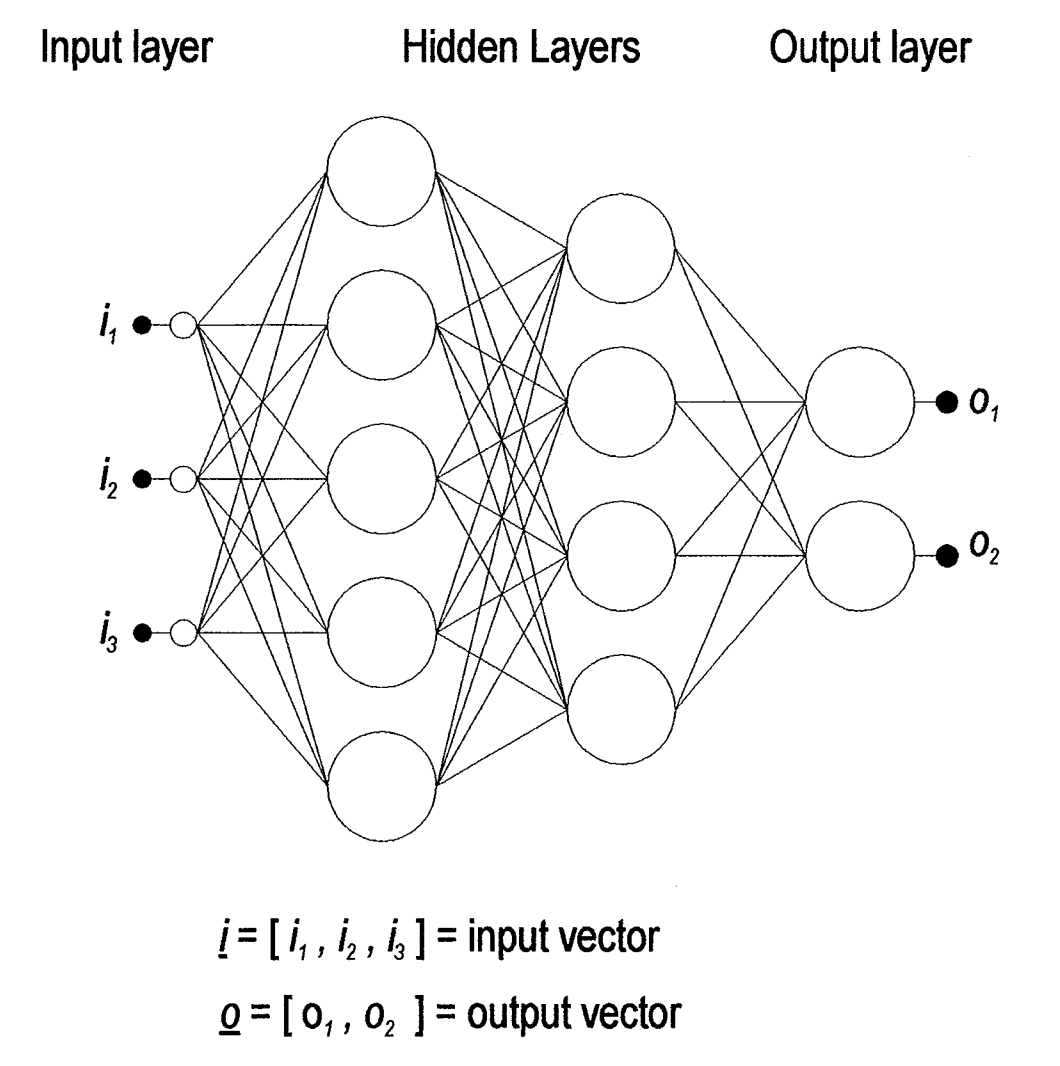
\includegraphics[width=8cm]{kapitel2/multilayerperc.png}
    \caption[Das mehrschichtige Perzeptron]{Das mehrschichtige Perzeptron mit zwei verborgenen Schichten, entnommen aus \cite*{Gardner1998}}
    
\end{figure}


\section{Sigmoid-Neuron}

Neben dem Perzeptron gibt es das \textit{Sigmoid} Neuron. Das Perzeptron gibt bekanntlich nur eine 0 oder eine 1 zurück. Es ist also eine Funktion nötig, die sich ohne \enquote{Diskontinuität}, schrittweise von 0 auf 1 ändert. Mathematisch bedeutet dies, dass eine stetige Funktion nötig ist, mit der die Ableitung berechnet werden kann. Dieses Problem kann überwunden werden, indem einen neuer Typ eines künstlichen Neurons eingeführt wird, der als \textit{Sigmoid-Neuron} bezeichnet wird. Sigmoid Neuronen ähneln Perzeptronen, sind jedoch so modifiziert, dass kleine Änderungen ihres Gewichts und ihres Bias nur eine geringe Änderung ihrer Leistung bewirken. Dies ist der Grund dafür, dass Netzwerke lernen können. \cite*[8]{Nielsen2015}.

%\begin{figure}[H]
 %   \centering
 %   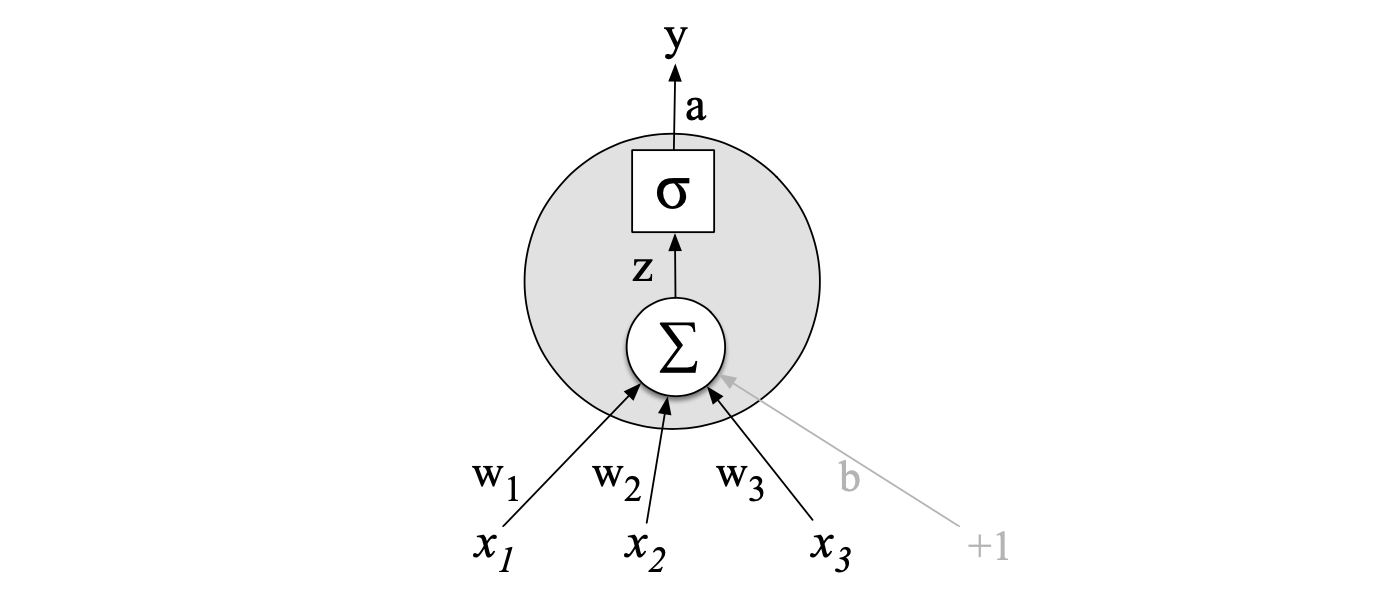
\includegraphics[width=11cm]{kapitel2/neuron.png}
  %  \caption[Eine neuronale Einheit]{Eine neuronale Einheit, die 3 Eingänge \textit{x1}, \textit{x2} und \textit{x3} (und eine Bias \textit{b}) hat und einen Ausgang \textit{y} erzeugt. Durch Summieren entsteht \textit{z}. Das Sigmoid nimmt \textit{z} ein und erzeugt \textit{a}. In diesem Fall ist die Ausgabe \textit{y} dieselbe wie \textit{a}, aber in tiefen Netzwerken wird \textit{y} vorbehalten, um die endgültige Ausgabe des gesamten Netzwerks zu berechnen. Entnommen aus \cite[125]{Jurafskya}}
   % \label{neurch2}
%\end{figure}


Genau wie ein Perzeptron hat das Sigmoid-Neuron die Eingaben $x_1, x_2, ...$, aber anstatt nur 0 oder 1 zu sein, können diese Eingänge auch beliebige Werte zwischen 0 und 1 annehmen. Also zum Beispiel 0,123 welches eine gültige Eingabe für ein Sigmoid-Neuron ist. Ebenso wie ein Perzeptron hat das Sigmoid-Neuron Gewichte für jede Eingabe, $w_1, w_2, ...$ und einen Bias, $b$. Die Ausgabe ist jedoch nicht 0 oder 1, stattdessen ist es $\sigma$, $(wx + b)$, wobei $\sigma$ als Sigmoidfunktion bezeichnet wird und durch Formel~\ref{SigmoidFu} definiert ist.

\begin{equation} \label{SigmoidFu}
    \sigma (z) = \frac{1}{1+e^{-z}}
\end{equation}

\myequations{Sigmoidfunktion}


\section{Aktivierungsfunktionen}
Ohne eine \textit{Aktivierungsfunktion} (auch als Nichtlinearität bezeichnet) würde die dichte Schicht (\enquote{dense layer}) nur aus zwei linearen Operationen bestehen - einem Punktprodukt und einer Addition: $Ausgabe = Punkt (w, Eingabe) + b$. Die Schicht könnte also nur lineare Transformationen, \enquote{affine Transformationen} der Eingabedaten lernen. Um Zugang zu einem viel umfangreicheren Hypothesenraum zu erhalten, wird eine Nichtlinearitäts- oder Aktivierungsfunktion benötigt \cite*[S. 72]{Chollet2017}.

\subsection{Sigmoid}
Die Sigmoidfunktion wird mit der Formel~\ref{Formel2_2} definiert und in der Abbildung~\ref{Kap2:Sigmoid_plot} dargestellt, die Ableitung der Sigmoidfunktion wird in der Formel~\ref{AbleitungSigm} definiert. Sie hat kleine Ausgangsänderungen im Bereich (0, 1), wenn der Eingang im Bereich $(-\infty, \infty)$ variiert. Mathematisch ist die Funktion stetig. Ein Neuron kann das Sigmoid zur Berechnung der nichtlinearen Funktion $\sigma(z = wx + b)$ verwenden. Wenn $z = wx + b$ sehr groß und positiv wird, dann wird $e^z \rightarrow 0$ also $\sigma(z) \rightarrow 1$, während wenn $z = wx + b$ sehr groß und negativ wird, wird $e^{-z} \rightarrow 0$ also $\sigma(z) \rightarrow 0$. Mit anderen Worten, ein Neuron mit Sigmoidaktivierung hat ein ähnliches Verhalten wie das Perzeptron, aber die Änderungen sind allmählich und Ausgabewerte wie 0,54321 oder 0,12345 sind vollkommen legitim. In diesem Sinne kann ein Sigmoid-Neuron auch mit \enquote{vielleicht} antworten \cite*[10]{AntonioGuili;AmitaKapoor;SujitPal2019}.

\begin{figure}[H]
    \centering
    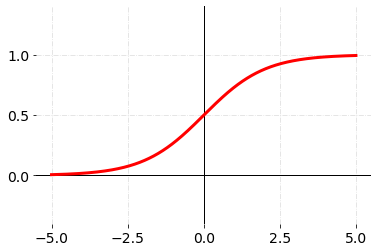
\includegraphics[width=8cm]{kapitel2/sig_plot.png}
    \caption[Darstellung der Sigmoid-Aktivierungsfunktion]{Darstellung der Sigmoid-Aktivierungsfunktion (eigene Darstellung)}
    \label{Kap2:Sigmoid_plot}
\end{figure}


\begin{equation} \label{AbleitungSigm}
    \begin{array}{ c }
        \sigma '(z)\ =\ \frac{d}{dz}\left(\frac{1}{1+e^{-z}}\right) =\frac{1}{\left( 1+e^{-z}\right)^{-2}}\frac{d}{dz} =\left( e^{-z}\right) \ =\frac{e^{-z}}{\left( 1+e^{-z}\right)}\frac{1}{\left( 1+e^{-z}\right)} \ =  \\
        \\
        \frac{e^{-z} +1-1}{\left( 1+e^{-z}\right)}\frac{1}{\left( 1+e^{-z}\right)} =\left(\frac{\left( 1+e^{-z}\right)}{\left( 1+e^{-z}\right)} -\frac{1}{\left( 1+e^{-z}\right)}\right)\frac{1}{\left( 1+e^{-z}\right)} = \\
        \\
        \left( 1-\frac{1}{\left( 1+e^{-z}\right)}\right)\left(\frac{1}{\left( 1+e^{-z}\right)}\right) =\ (1-\sigma (z))\sigma (z)
    \end{array}
\end{equation}
\label{AbleitungSigm}
\myequations{Ableitung der Sigmoidfunktion}

\subsection{Tanh}
Die Tanh-Aktivierungsfunktion wird mit der Formel~\ref{TanhF} definiert ihre Ableitung wird in der Formel~\ref{TanhAbl} berechnet. Sie hat ihre Ausgangsänderungen im Bereich (-1, 1). Sie hat eine Struktur, die der Sigmoid-Funktion sehr ähnlich ist. Der Vorteil gegenüber der Sigmoidfunktion besteht darin, dass ihre Ableitung steiler ist, was bedeutet, dass sie mehr Werte enthalten kann (vergleiche Abbildung~\ref{Kap2:Tanh_plot}). Für die Ableitung der Tanh-Aktivierungsfunktion gilt, $e^z = \frac{d}{dz}e^z$ und $e^{-z} = \frac{d}{dz}e^{-z}$.

\begin{equation} \label{TanhF}
    tanh(z) = \frac{e^{z}-e^{-z}}{e^{z}-e^{-z}}
\end{equation}
\myequations{Die Tanh-Funktion}

\begin{equation} \label{TanhAbl}
    \begin{array}{ c }
        \frac{d}{dz} tanh( x) =\frac{\left( e^{z} +e^{-z}\right)\left( e^{z} +e^{-z}\right) -\left( e^{z} -e^{-z}\right)\left( e^{z} -e^{-z}\right)}{\left( e^{z} +e^{-z}\right)^{2}} = \\
        \\
        1-\frac{\left( e^{z} -e^{-z}\right)^{2}}{\left( e^{z} +e^{-z}\right)^{2}} \ =\ 1\ -tanh^{2}( z)
    \end{array}
\end{equation}
\myequations{Die Ableitung der Tanh-Funktion}

\begin{figure}[H]
    \centering
    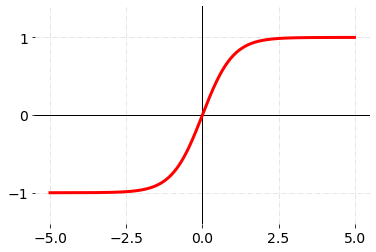
\includegraphics[width=8cm]{kapitel2/tanh_plot.png}
    \caption[Darstellung der Tanh-Aktivierungsfunktion]{Darstellung der Tanh-Aktivierungsfunktion (eigene Darstellung)}
    \label{Kap2:Tanh_plot}
\end{figure}

\subsection{ReLu}
Die ReLu ist eine relativ einfache Funktion, sie ist relativ neu und wird sehr häufig verwendet \cite*[11]{AntonioGuili;AmitaKapoor;SujitPal2019}. Sie wird in Formel~\ref{Relu} definiert, die zugehörige Ableitungsfunktion wird in der Formel~\ref{ReluAbl} berechnet. Wie in Abbildung~\ref{Kap2:ReLu_plot} zu sehen, ist die Funktion für negative Werte Null und wächst für positive Werte linear. Die ReLU ist relativ einfach zu implementieren.

\begin{equation} \label{Relu}
    f( x) \ =\ \begin{cases}
        0 & wenn\ x\  <\ 0    \\
        x & wenn\ x\  \geq\ 0 \\
    \end{cases}
\end{equation}
\myequations{Die ReLu-Funktion}

\begin{equation} \label{ReluAbl}
    f'( x) \ =\ \begin{cases}
        1, & wenn\ x\  >\ 0 \\
        0, & sonst
    \end{cases}
\end{equation}
\myequations{Die Ableitung der ReLu-Funktion}

\begin{figure}[H]
    \centering
    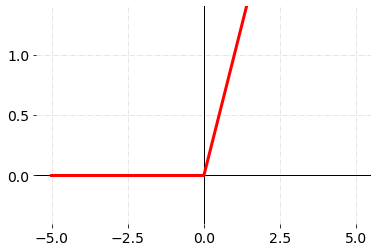
\includegraphics[width=8cm]{kapitel2/relu_plot.png}
    \caption[Darstellung der ReLu-Aktivierungsfunktion]{Darstellung der ReLu-Aktivierungsfunktion (eigene Darstellung)}
    \label{Kap2:ReLu_plot}
\end{figure}

\subsection{softmax}
Die grundlegende Schwierigkeit bei der Durchführung kontinuierlicher Mathematik auf einem digitalen Computer besteht darin, dass unendlich viele reelle Zahlen mit einer endlichen Anzahl von Bitmustern dargestellt werden müssen. Dabei entstehen Rundungsfehler die problematisch sein können, insbesondere wenn sie sich über viele Operationen hinweg zusammensetzen. Sie führen dazu, dass theoretisch funktionierende Algorithmen in der Praxis fehlschlagen. Ein Beispiel für eine Funktion, die gegen Rundungsfehler stabilisiert, ist die softmax-Funktion \cite*[80-81]{IanGoodfellowYoshuaBengio2016}.

\begin{equation} \label{FormelSoft}
    softmax( x)_{i} =\frac{exp( x_{i})}{\sum ^{n}_{j=1} exp( x_{j})}
\end{equation}
\myequations{Die softmax-Funktion}

\section{Optimierungsalgorithmen}
Die meisten Deep-Learning-Algorithmen beinhalten irgendeine Art von Optimierung. Optimierung bezieht sich auf die Aufgabe, eine Funktion $f(x)$ durch Ändern von $x$ entweder zu minimieren oder zu maximieren. Die meisten Optimierungsprobleme werden in Bezug auf Minimierung von $f(x)$ formuliert. Die Maximierung kann über einen Minimierungsalgorithmus durch Minimieren von $-$$f(x)$ erreicht werden. Die Funktion die minimiert oder maximiert werden soll, wird als \textit{Objektive Funktion} bezeichnet. Es wird auch \textit{Kostenfunktion} oder \textit{Verlustfunktion} bezeichnet. Zum Beispiel ist die Funktion $x^{*} = arg\ min\ f( x)$ eine solche Funktion.

\subsection{Gradientenabstiegsverfahren}
Der Gradientenabstiegsverfahren ist einer der beliebtesten Algorithmen zur Optimierung neuronaler Netze. Der Gradientenabstiegsverfahren ist ein Weg, um eine Zielfunktion $J(\theta)$ zu minimieren, die durch die Parameter eines Modells $\theta \in \mathbb{R}^{d}$ parametrisiert wird. Die Parameter werden in der entgegengesetzten Richtung des Gradienten der Zielfunktion $\nabla \theta J (\theta)$ angepasst. Die Lernrate $\eta$ bestimmt die Größe der Schritte, die unternommen werden, um ein lokales Minimum zu erreichen. Mit anderen Worten, wird der Richtung bergab gefolgt, die durch die Zielfunktion erzeugt wird, bis ein \enquote{Tal} erreicht wird (siehe Abbildung~\ref{Kap2:Grad}) \cite*{Ruder2016}.



\begin{figure}[H]
    \centering
    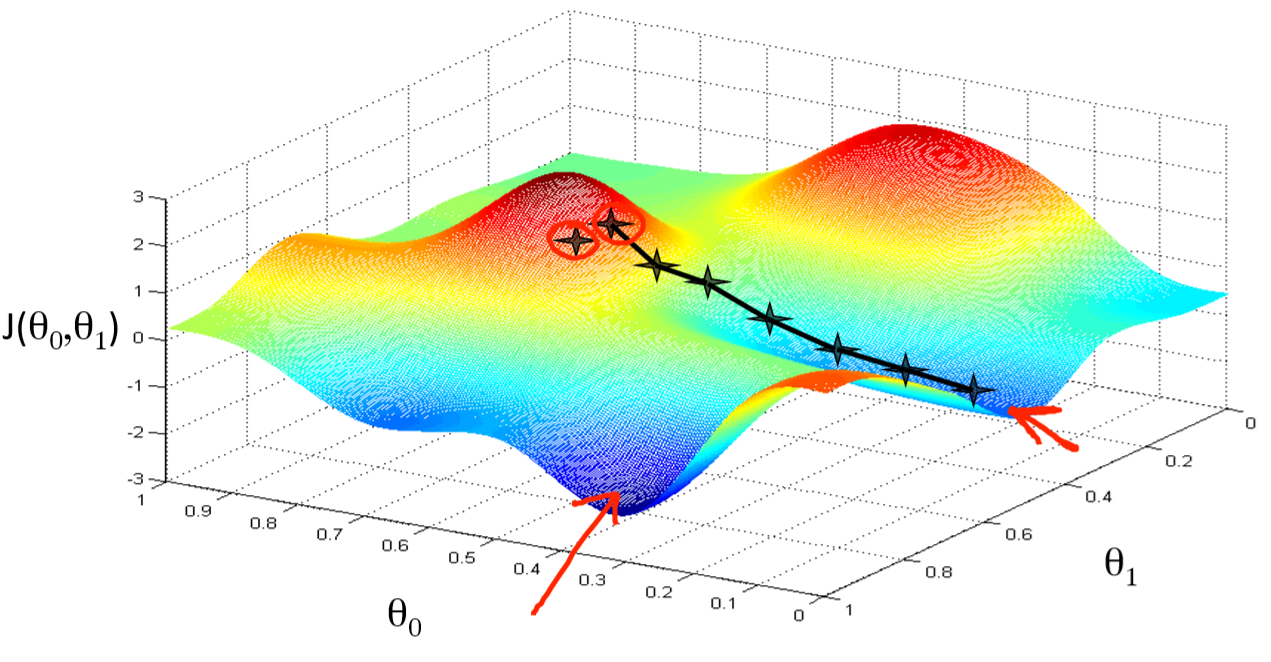
\includegraphics[width=12cm]{kapitel2/gradient.png}
    \caption[Der Gradientenabstiegsverfahren]{Darstellung des Gradientenabstiegsverfahren, entnommen aus \cite*{hackernoon}.}
    \label{Kap2:Grad}
\end{figure}



\subsection{Batch Gradientenabstiegsverfahren}
Der Standard Gradientenabstiegsverfahren, auch Batch Gradientenabstiegsverfahren genannt, berechnet den Gradienten der Verlustfunktion zu den Parametern $\theta$ für den gesamten Trainingsdatensatz.


\begin{equation} \label{FormelGradBatch}
    \theta = \theta - \eta \cdot \nabla_{\theta}J(\theta)
\end{equation}
\myequations{Der Gradientenabstiegsverfahren}

Da der gesamte Datensatz berechnet werden muss, um nur eine Aktualisierung durchzuführen, kann der Batch Gradientenabstiegsverfahren sehr langsam sein und ist für Datensätze, die nicht in den Speicher passen, nicht zu handhaben. Der Batch Gradientenabstiegsverfahren ermöglicht es auch nicht, das Modell mit neuen Beispielen im laufenden Betrieb zu aktualisieren \cite*{Ruder2016}.

\subsection{Stochastische Gradientenabstiegsverfahren}

Im Gegensatz dazu führt der stochastische Gradientenabstiegsverfahren (SGD) eine Parameteraktualisierung für jedes Trainingsbeispiel durch. Der Batch Gradientenabstiegsverfahren führt redundante Berechnungen für große Datenmengen durch, da Gradienten für ähnliche Beispiele vor jeder Parameteraktualisierung neu berechnet werden. Der stochastische Gradientenabstiegsverfahren beseitigt diese Redundanz, indem jeweils ein Update durchgeführt wird. Es ist daher in der Regel viel schneller und kann auch beim laufendem Lernen verwendet werden \cite*{Ruder2016}.

\begin{equation} \label{FormelGradStoch}
    \theta = \theta - \eta \cdot \nabla_{\theta}J(\theta;x^{(i)};y^{(i)})
\end{equation}
\myequations{Der stochastische Gradientenabstiegsverfahren}



\section{Backpropagation}
Das \textit{Backpropagation-Verfahren} bezieht sich auf die Gewichte eines mehrschichtigen Netzes und wendet dabei praktisch die Anwendung der Kettenregel der Differentialrechnung an. Es wird vom Gradienten in Bezug auf die Ausgabe (oder die Eingabe der Nachfolge) rückwärts gearbeitet. Die Kettenregel sagt dabei aus, wie zwei kleine Effekte (eine kleine Änderung von $x$ auf $y$ und der von $y$ auf $z$) zusammengesetzt sind. Eine kleine Änderung von $\Delta y$ in $x$ wird zuerst in eine kleine Änderung $\Delta y$ in $y$ umgewandelt, indem sie mit $\frac{\partial y}{\partial y}$  multipliziert wird (die partielle Ableitung). In ähnlicher Weise erzeugt die Änderung $\Delta y$ eine Änderung von $\Delta z$ in $z$ (siehe Formel~\ref{ChainRule}) \cite*{Lecun2015}.

\begin{gather} \label{ChainRule}
    \Delta z =  \frac{\partial z}{\partial y} \Delta y \notag\\
    \Delta y = \frac{\partial y}{\partial x} \Delta x \notag\\
    \Delta z = \frac{\partial z}{\partial y}\frac{\partial y}{\partial x} \Delta x \notag\\
    \frac{\partial z}{\partial x} = \frac{\partial z}{\partial y} \frac{\partial y}{\partial x}
\end{gather}
\myequations{Backpropagation}

Die Gleichungen, die zur Berechnung des Vorwärtsdurchlaufs (siehe Abbildung~\ref{BackProp}) in einem neuronalen Netz mit zwei verborgenen Schichten und einer Ausgangsschicht verwendet werden, bilden jeweils ein Modul, durch das man Gradienten zurück propagieren kann. Auf jeder Ebene wird zuerst die Gesamteingabe $z$ für jede Einheit berechnet. Dann wird eine nichtlineare Funktion auf $z$ angewendet, um die Ausgabe der Einheiten zu erhalten. Eine nichtlineare Funktion kann z.B. eine ReLu- oder eine Sigmoid-Funktion oder eine tanh-Funktion sein. Im Rückwärtsdurchlauf (siehe Abbildung~\ref{BackProp}) wird in jeder verborgenen Schicht die Ableitung der Fehler in Bezug auf die Ausgabe jeder Einheit berechnet. Dies geschieht durch Vergleichen der Ausgaben mit der richtigen Antwort \cite*{Lecun2015}.


\begin{figure}[H]
    \centering
    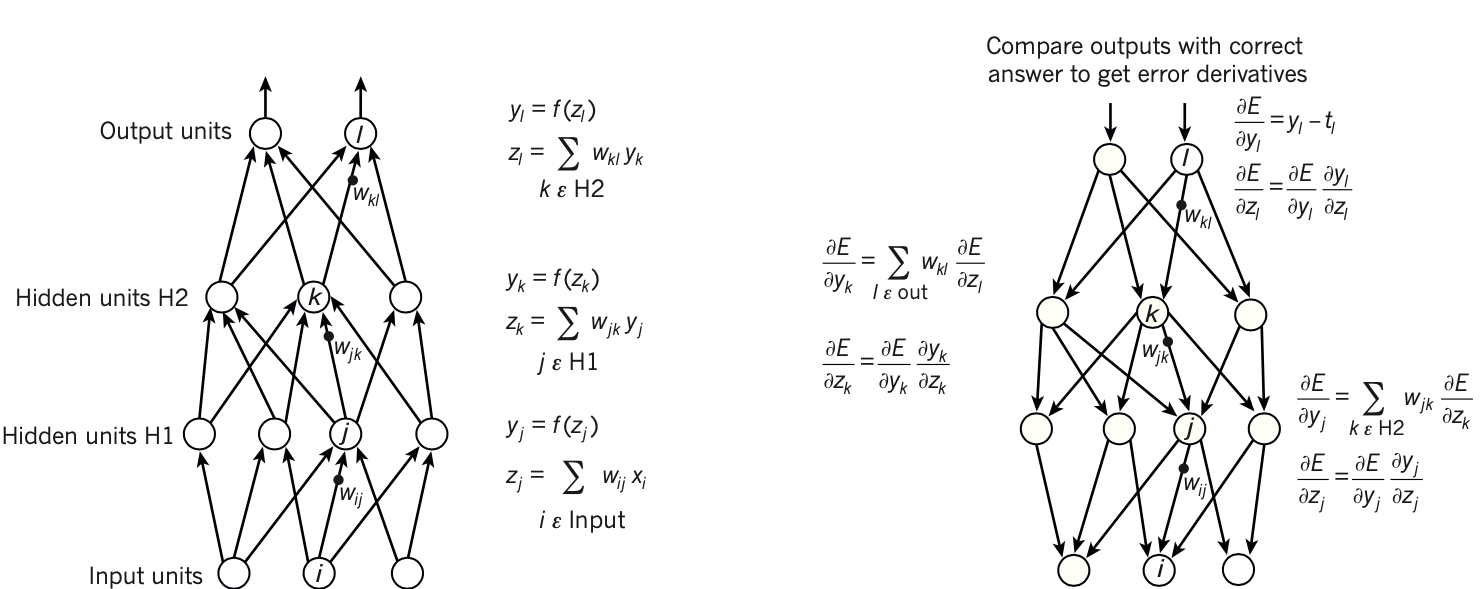
\includegraphics[width=13cm]{kapitel2/backprop.png}
    \caption[Die Vorwärts- und Rückwärtsschritte im Backpropagation]{Darstellung vergleicht die Schritte des Backpropagation Verfahrens nach vorne und hinten (in Anlehnung an \cite*{Lecun2015}).}
    \label{BackProp}
\end{figure}

Die Backpropagation-Gleichung wird wiederholt angewendet. Der Rückwärtsdurchlauf bezieht sich auf die Idee, die Differenz zwischen Vorhersage- und Istwerten zu verwenden, um die Hyperparameter der verwendeten Methode anzupassen. Für die Anwendung ist jedoch immer eine vorherige \enquote{Vorwärtspropagation} erforderlich.


\section{Lernrate im Deep Learning}\label{learnsection}
Die \textit{Lernrate} beeinflusst den Betrag, um den die Parameter während der Optimierung angepasst werden, um den Fehler des neuronalen Netzwerks zu minimieren. Es ist ein Koeffizient, der die Größe der Schritte (Aktualisierungen) skaliert, die ein neuronales Netzwerk auf seinen Parameter (Vektor $x$) ausführt, wenn es den Funktionsraum der Verlustfunktion durchquert. Ein großer Koeffizient (z. B. 1) lässt die Parameter Sprünge machen, und kleine (z. B. 0,00001) lassen ihn langsam voranschreiten. Im Gegensatz dazu sollten kleine Lernraten letztendlich zu einem Fehlerminimum führen (es kann eher ein lokales als ein globales Minimum sein). Sehr kleine Lernraten können mehr Zeit zum Lernen in Anspruch nehmen und die Belastung eines bereits rechenintensiven Prozesses erhöhen  \cite*[77]{Patterson2019}.


\begin{figure}[H]
    \centering
    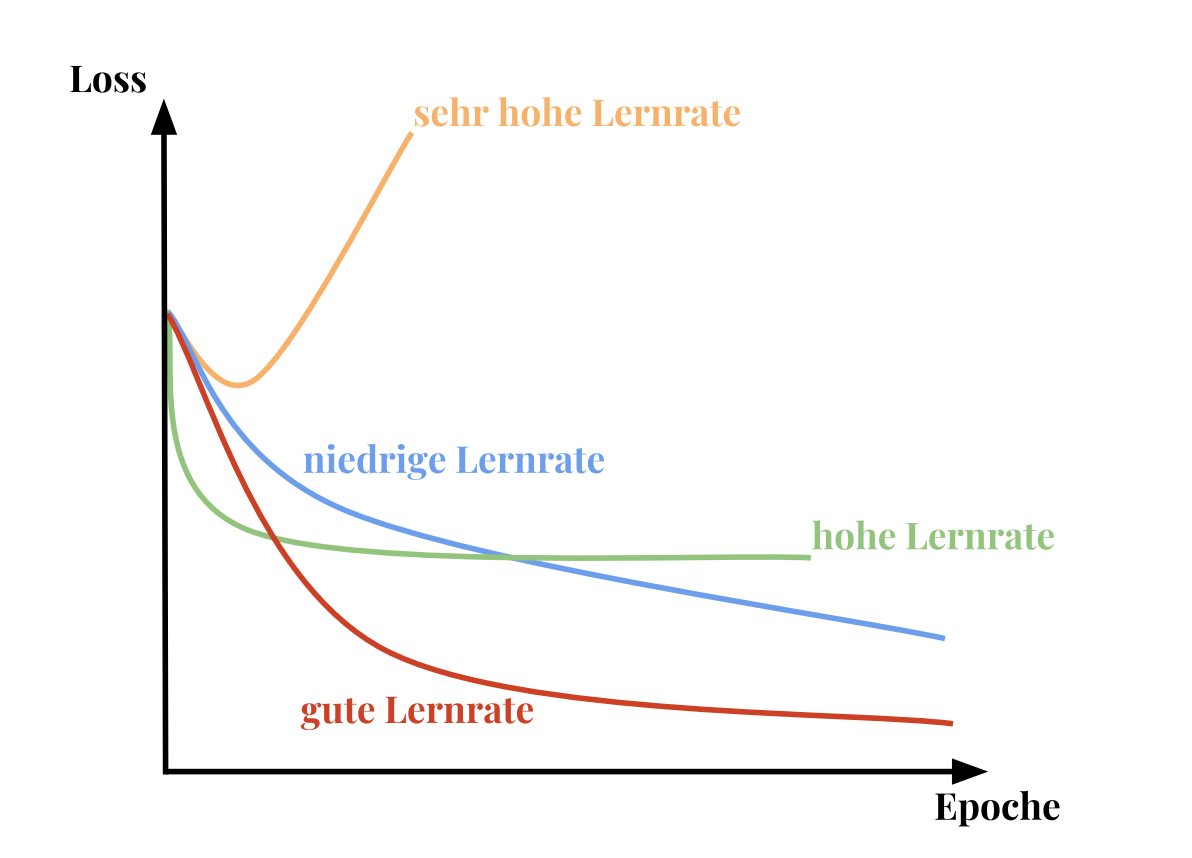
\includegraphics[width=10cm]{kapitel2/learnrate.png}
    \caption[Einfluss der Lernrate auf den Verlust]{Vergleich unterschiedlicher Lernraten und deren Effekte auf den Verlust. Bei niedrigen Lernraten ist eine \enquote{lineare} Verbesserungen zu sehen. Mit hohen Lernraten werden sie exponentieller. Höhere Lernraten verringern den Verlust schneller, bleiben jedoch bei schlechteren Verlustwerten hängen (grüne Linie). Dieses liegt daran, dass die Optimierung zu viel \enquote{Energie} enthält und die Parameter \enquote{chaotisch herum springen} und sich nicht an einem Ort in der \enquote{Optimierungslandschaft} niederlassen können (in Anlehnung an \cite*{StanfordUniversityCoursecs231n2018}). }
    \label{Kap2:Lern}
\end{figure}

\section{Unteranpassung und Überanpassung}\label{overundersec}
Optimierungsalgorithmen versuchen zunächst, das Problem der \textit{Unteranpassung} (\enquote{Underfitting}) zu lösen. Das heißt, eine Linie zu nehmen, die sich den Daten nicht gut annähert, und sie besser an die Daten heranzuführen. Eine gerade Linie, die über ein gekrümmtes Streudiagramm schneidet, wäre ein gutes Beispiel für eine \textit{Unteranpassung}, wie in Abbildung~\ref{Kap2:OverUnder} dargestellt. Wenn die Linie zu gut zu den Daten passt, besteht das  gegenteilige Problem, welches als \textit{Überanpassung} (\enquote{Overfitting}) bezeichnet wird \cite*[27]{Patterson2019}.

\begin{figure}[H]
    \centering
    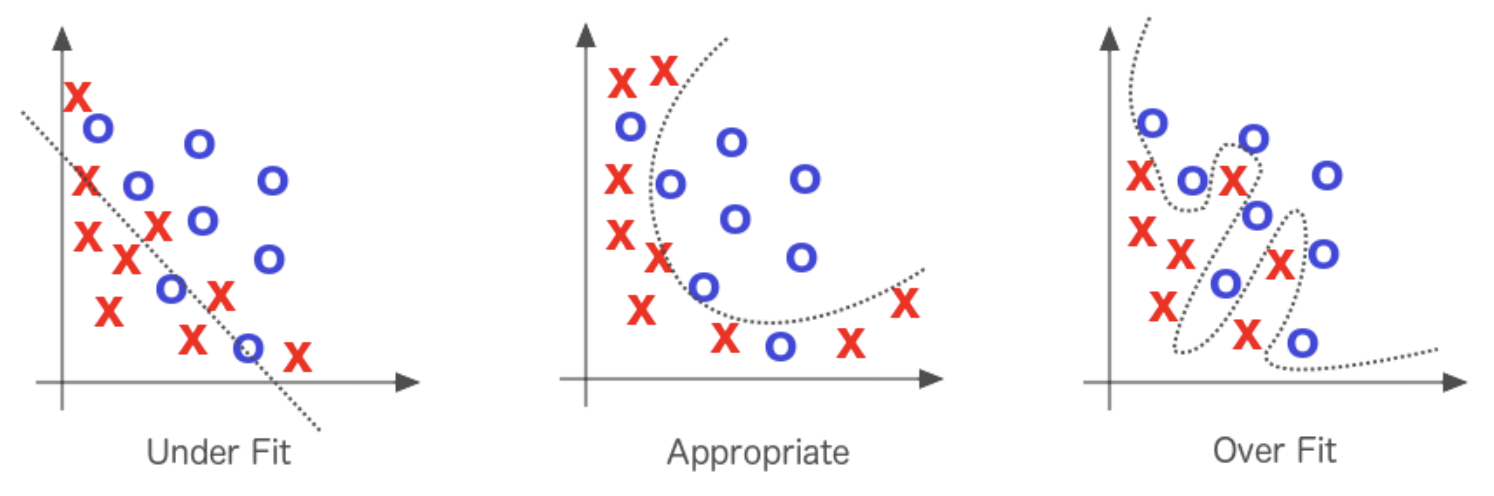
\includegraphics[width=10cm]{kapitel2/overundefit.png}
    \caption[Vergleich der Unteranpassung mit der Überanpassung]{Die Abbildung vergleicht die Überanpassung mit der Unteranpassung. Die einzelnen Punkte passen sich dem trainierten Modell zu sehr an, der Verlust wird also so klein, dass das Modell nicht mehr zuverlässige Ergebnisse liefern kann. Dies ist darauf zurückzuführen, dass das Modell \enquote{zu viel} aus dem Trainingsdatensatz gelernt hat. Unteranpassung ist der Fall, wenn das Modell aus den Trainingsdaten \enquote{nicht genug gelernt} hat, was zu einer geringen Verallgemeinerung und unzuverlässigen Vorhersagen führt (Grafik entnommen aus \cite*[27]{Patterson2019}). }
    \label{Kap2:OverUnder}
\end{figure}

\section{Regularisierung}\label{regSec}
Die Regularisierung lässt die Auswirkungen von außer Kontrolle geratenen Parametern minimieren, indem verschiedene Methoden oder Strategien verwendet werden, um die Parametergröße im Laufe der Zeit zu minimieren. Der Hauptzweck der Regularisierung besteht darin, die Überanpassung zu kontrollieren \cite*[79]{Patterson2019}.

Ein zentrales Problem beim maschinellen Lernen besteht darin, einen Algorithmus zu erstellen, der nicht nur bei den Trainingsdaten, sondern auch bei neuen Eingaben eine gute Leistung erbringt. Viele beim maschinellen Lernen verwendete Strategien sind explizit darauf ausgelegt, den Testfehler zu reduzieren, möglicherweise auf Kosten eines erhöhten Trainingsfehlers. Die Strategien zur Vorbeugung dieser Probleme werden zusammen als Regularisierung bezeichnet. Tatsächlich war die Entwicklung effektiverer Regularisierungsstrategien eine der wichtigsten Forschungsanstrengungen auf diesem Gebiet. Regularisierung kann schließlich definiert werden als \enquote{jede Änderung, die wir an einem Lernalgorithmus vornehmen, um dessen Generalisierungsfehler, aber nicht seinen Trainingsfehler zu reduzieren} \cite*[228]{IanGoodfellowYoshuaBengio2016}.

\subsection{Early Stopping}
Wenn große Modelle trainiert werden, um eine bestimmte Aufgabe zu lösen, wird häufig festgestellt, dass der Trainingsfehler mit der Zeit stetig abnimmt, der Fehler des Validierungssatzes jedoch wieder zunimmt. Dies bedeutet, dass ein Modell mit einem besseren Validierungsfehler (und damit einem besseren Testfehler) erhalten werden kann, indem zu dem Zeitpunkt mit dem niedrigsten Validierungsfehler zur Parametereinstellung zurückgekehrt wird. Jedes Mal, wenn sich der Fehler der Validierung verbessert, wird eine Kopie der Modellparameter gespeichert. Wenn der Trainingsalgorithmus beendet wird, wird diese Parameter anstelle der neuesten Parameter zurückgegeben. Diese Strategie wird als \textit{Early Stopping} \enquote{frühes Stoppen} bezeichnet. Es ist wahrscheinlich die am häufigsten verwendete Form der Regularisierung. Seine Popularität ist sowohl auf seine Wirksamkeit als auch auf seine Einfachheit zurückzuführen \cite*[246]{IanGoodfellowYoshuaBengio2016}.


\subsection{Dropout}
Eine weitere Strategie um Überanpassung zu vermeiden wird in \cite*{Srivastava2014} dargestellt. \textit{Dropout} bietet eine rechnerisch kostengünstige, aber leistungsstarke Methode zur Regularisierung dar. Es ist das aufteilen des Netzwerkes in mehreren Teile. Es wird also ein Ensemble aus diesen kleinen Teilen (\enquote{sub-networks}) gebildet \cite*[258]{IanGoodfellowYoshuaBengio2016}.



\begin{figure}[H]
    \centering
    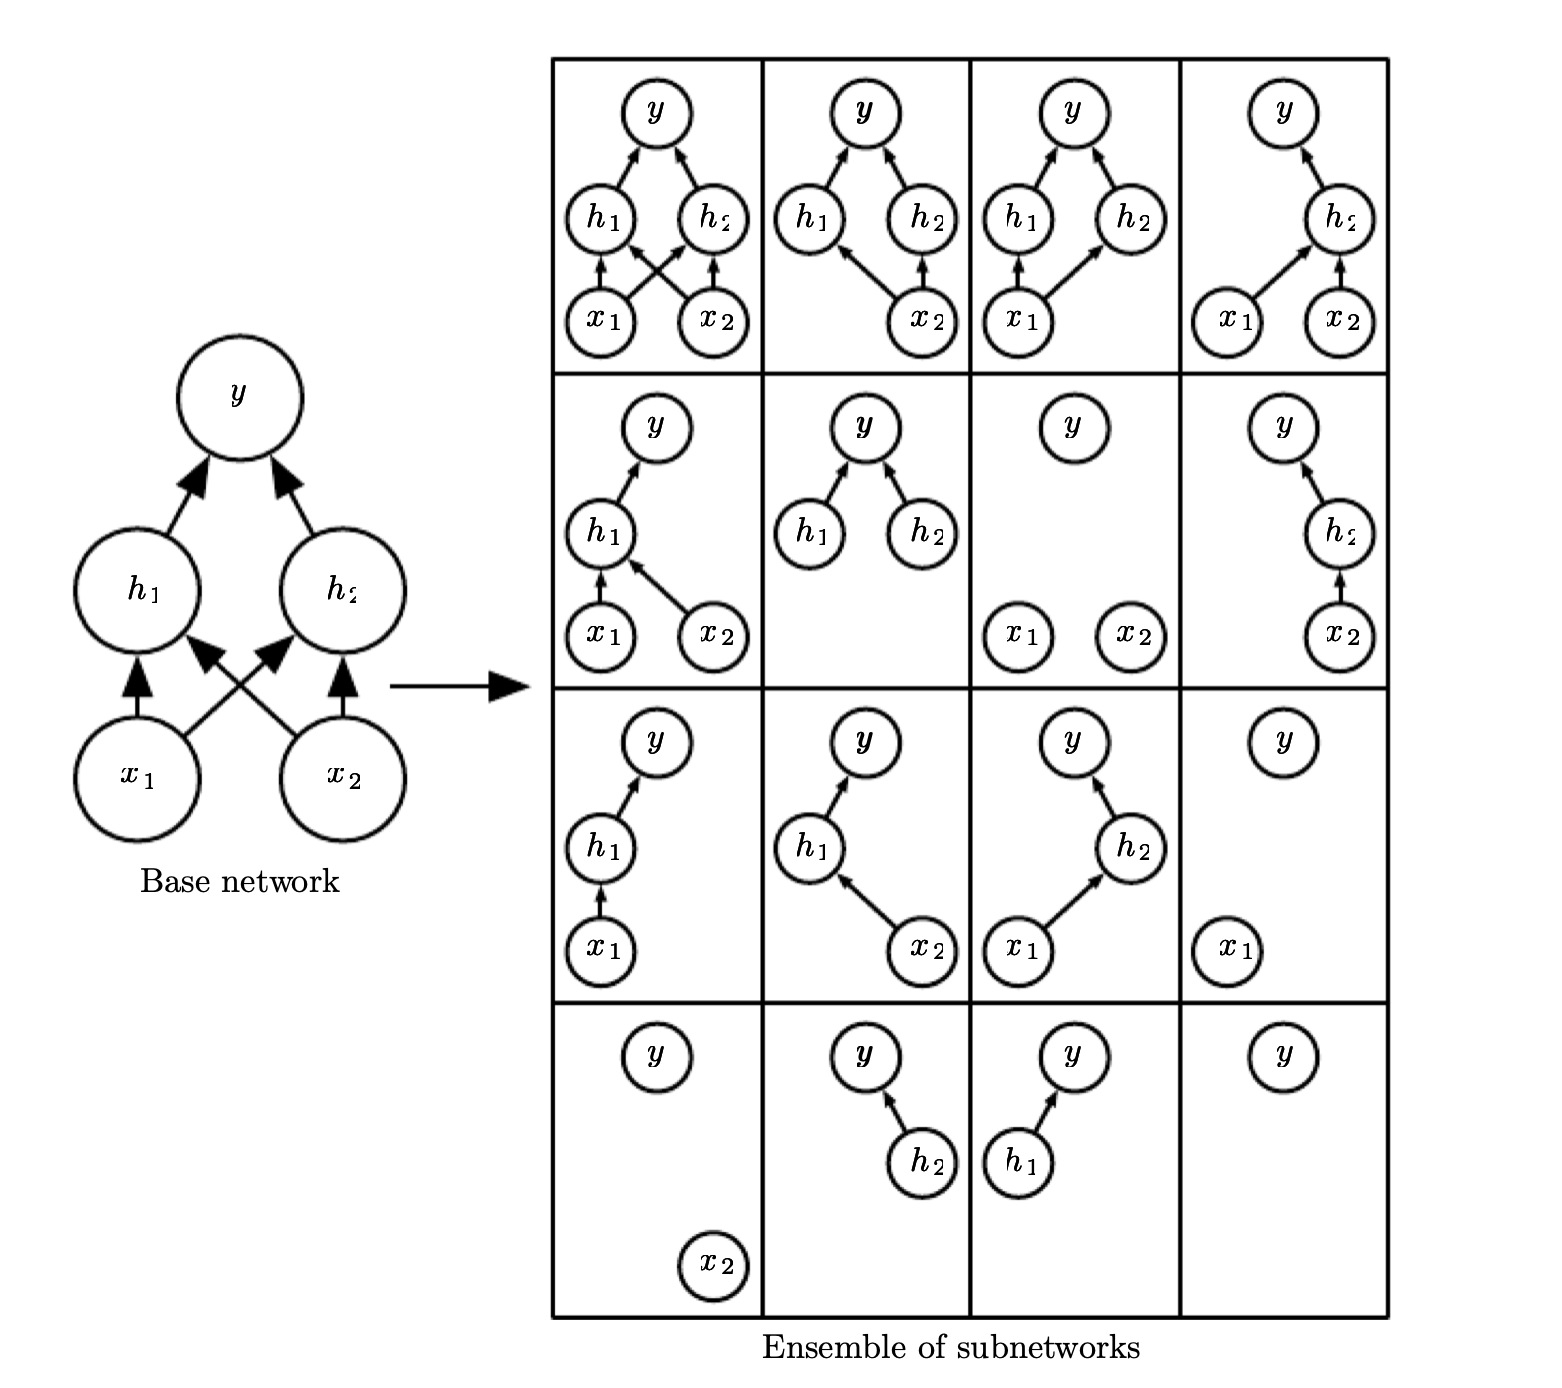
\includegraphics[width=10cm]{kapitel2/dropout.png}
    \caption[Dropout]{Dropout trainiert ein Ensemble. Ein Ensemble besteht aus allen Teilnetzwerken. Es wird durch das entfernen von Einheiten aufgebaut. Das Ensemble besteht aus 16 Teilmengen, aus den vier Einheiten des Basis-Netzwerks. Die 16 Subnetze werden durch das Löschen verschiedener Teilmengen von Einheiten aus dem ursprünglichen Netzwerk gebildet (entnommen aus \cite*[260]{IanGoodfellowYoshuaBengio2016}).}
    \label{Kap2:Dropout}
\end{figure}

\subsection{L1 und L2}
Eine weitere Strategie der Regularisierung ist die Modifikation der \textit{L1} und \textit{L2} Gewichte. Beim Deep Learning wird die Größe von Vektoren, mit einer Funktion, die als \enquote{Norm} bezeichnet wird, \cite*[39]{IanGoodfellowYoshuaBengio2016} gemessen. Formal ist diese Norm $L^p$ definiert als:

\begin{equation} \label{FormelNorm2}
    \Vert x\Vert \ =\ \left(\sum _{i}\bigr| x_{i}\bigr|^{p}\right)^{\frac{1}{p}}.
\end{equation}
\myequations{Regularisierung}

Normen, einschließlich der $L^p$-Norm, sind Funktionen, die Vektoren auf nicht negative Werte abbilden. Auf einer intuitiven Ebene misst die Norm eines Vektors $x$ den Abstand vom Ursprung zum Punkt $x$. Die $L^2$-Norm mit $p = 2$ ist als euklidische Norm bekannt. Es ist der euklidische Abstand vom Ursprung zum Punkt $x$. Die $L^2$-Norm wird beim maschinellen Lernen häufig verwendet, sie wird als $\Vert x\Vert$ bezeichnet, wobei der Index 2 weggelassen wird \cite*[39]{IanGoodfellowYoshuaBengio2016}.

Wenn zwischen Elementen zu unterscheiden ist, die genau Null sind und Elementen die klein, aber ungleich Null sind, wird die $L^1$-Norm angewendet. Die $L^1$-Norm kann vereinfacht werden als \cite*[40]{IanGoodfellowYoshuaBengio2016}:

\begin{equation} \label{FormelNorm1}
    \Vert x\Vert 1\ =\ \sum _{i}\bigr| x_{i}\bigr|.
\end{equation}
\myequations{L1-Regularisierung}

\section{Metriken im Deep Learning}
Im Deep Learning werden oftmals Klassifizierungsprobleme gelöst. In diesem Abschnitt werden die wichtigsten Metriken für das Messen solcher Probleme definiert.
\paragraph{Precision}
Precision (Präzision) gibt die Häufigkeit an, mit der ein Modell bei der Vorhersage der positiven Klasse korrekt war. Das ist:

\begin{equation} \label{Preci}
             Precision =  \frac{True\ Positives}{True\ Positives\ + False\ Positives}.
        \end{equation}
        \myequations{Precision}
        
\paragraph{Recall}
Ist eine Metrik, die folgende Frage beantwortet: Wie viele der möglichen positiven Bezeichnungen hat das Modell korrekt identifiziert? Es wird definiert durch:
\begin{equation} \label{Recall}
             Recall =  \frac{True\ Positives}{True\ Positives\ + False\ Negatives}.
        \end{equation}
        \myequations{Recall}


\paragraph{F1-Score}
Der F1-Score ist das harmonische Mittel der Precision und des Recalls. Es wird mit folgender Formel berechnet:
\begin{equation} \label{F1Score}
             F_1 =  2 \cdot \frac{Precision\ \cdot Recall}{Precision\  + Recall}.
        \end{equation}
        \myequations{F1-Score}
        

\section{Verlustfunktion und Kreuzentropie}
\subsection{Verlustfunktionen}
Innerhalb eines neuronalen Netzwerks wandelt eine \textit{Verlustfunktion} oder auch \textit{Kostenfunktion} genannt, alle möglichen Fehler in eine Zahl um, um den Gesamtfehler des Netzwerks darzustellen. Im Wesentlichen ist es ein Maß dafür, wie falsch ein Netzwerk liegt.

Das Neuron lernt dadurch, indem es Gewichte und Bias mit einer Rate ändert, die durch die partiellen Ableitungen der Kostenfunktion $\partial$$C$/$\partial$$w$ und $\partial$$C$/$\partial$$b$ bestimmt wird. Zu sagen, dass das \enquote{Lernen langsam ist}, ist also dasselbe wie zu sagen, dass diese partiellen Ableitungen klein sind \cite*[61]{Nielsen2015}. Gegeben sei die quadratische Verlustfunktion:

\begin{equation} \label{Formel2_5}
    C=\frac{( y-a)^{2}}{2},
\end{equation}
\myequations{Kostenfunktion}

dabei ist $a$ die Ausgabe des Neurons, wenn die Eingabe des Trainings $x = 1$ ist, und $y = 0$ die entsprechende gewünschte Ausgabe. Um dies in Bezug auf Gewicht und Bias expliziter zu schreiben, sei daran erinnert, dass $a = \sigma(z)$ ist, wobei $z = wx + b$ ist. Es ergeben sich durch die Anwendung der Kettenregel folgende Gleichungen:

\begin{equation} \label{Formel2_6}
    \frac{\partial C}{\partial w} =( a-y) \sigma '( z) x=a\sigma '( z)
\end{equation}
\myequations{Partielle Kostenfunktion der Gewichte}

\begin{equation} \label{Formel2_7}
    \frac{\partial C}{\partial b} =( a-y) \sigma '( z) =a\sigma '( z).
\end{equation}
\myequations{Partielle Kostenfunktion des Bias}
        
Aus der Abbildung~\ref{Kap2:Sigmoid_plot} ist die Kurve der Sigmoidfunktion zu sehen. Die Kurve wird sehr flach, wenn der Ausgang des Neurons nahe bei 1 liegt, und daher wird $\sigma'(z)$ sehr klein. Die Gleichungen~\ref{Formel2_6} und ~\ref{Formel2_7} sagen dann aus, dass $\partial$$C$/$\partial$$w$  und  $\partial$$C$/$\partial$$b$ sehr klein werden. Dies ist der Grund warum das lernen langsamer wird.

\subsection{Kreuzentropie}
Nach \cite*[62]{Nielsen2015} kann die Lernverlangsamung gelöst werden, indem die quadratische Verlustfunktion durch eine andere Verlustfunktion ersetzt wird. Diese Funktion wird als als \textit{Kreuzentropie} bezeichnet. Die Abbildung~\ref{Kap2:Entropie} zeigt die Kreuzentropie mit mehreren Eingabevariablen und entsprechenden Gewichten und Bias. Die Ausgabe des Neurons ist $a = \sigma(z)$, wobei $z =  \sum _{j} w_{j} b_{j} + b$ ist, die gewichtete Summe des Inputs. Die Kreuzentropie Kostenfunktion für dieses Neuron wird definiert durch:

\begin{equation} \label{Formel2_8}
    C=\ -\frac{1}{n}\sum _{x}[ y\ ln\ a\ +\ ( 1-y) \ ln( 1-a)]
\end{equation}
\myequations{Kreuzentropie Kostenfunktion}

wobei $n$ die Gesamtzahl der Trainingselemente darstellt. Die Summe gibt die entsprechende gewünschte Ausgabe $x$ und $y$ über alle Trainingseingaben an. Zusammenfassend ist die Kreuzentropie positiv und tendiert gegen Null, wenn das Neuron
\enquote{besser} wird, bei der Berechnung der gewünschten Ausgabe $y$ für alle Trainingseingaben $x$.  Die Kostenfunktion hat jedoch den Vorteil, dass sie im Gegensatz zu der quadratischen Kostenfunktion das Problem der Verlangsamung des Lernens vermeidet. Um dies näher zu beschreiben, soll die partielle Ableitung der Kreuzentropie in Bezug auf die Gewichte berechnet werden \cite*[63]{Nielsen2015}.

\begin{gather} \label{Formel2_9}
    \frac{\partial C}{\partial w_{j}} =-\frac{1}{n}\sum _{x}\left(\frac{y}{\sigma ( z)} -\frac{1-y}{1-\sigma ( z)}\right)\frac{\partial \sigma }{\partial w_{j}} = \notag\\
    -\frac{1}{n}\sum _{x}\left(\frac{y}{\sigma ( z)} -\frac{1-y}{1-\sigma ( z)}\right) \sigma '( z) x_{j}
    \notag\\
    \frac{\partial C}{\partial w_{j}} \ =\ \frac{1}{n}\sum _{x}\frac{\sigma '( z) x_{j}}{\sigma ( z)( 1-\sigma ( z))}( \sigma ( z) -y)
    \notag\\
    \frac{\partial C}{\partial w_{j}} \ =\ \frac{1}{n}\sum _{x} x_{j}( \sigma ( z) -y)
\end{gather}
\myequations{Herleitung der Kreuzentropie}

Die Geschwindigkeit, mit der das Gewicht $w$ lernt, wird durch $\sigma(z) - y$ gesteuert, also durch den Fehler in der Ausgabe. Je größer dieser Fehler wird, desto schneller lernt das Neuron. Dies ist ein gewünschtes Verhalten. Insbesondere wird die Lernverlangsamung vermieden, die durch den Term $\sigma'(z)$ in der analogen Gleichung für die quadratische Kostenfunktion~\ref{Formel2_6} verursacht wird. Wenn die Kreuzentropie verwendet wird, wird der Term $\sigma'(z)$ aufgehoben und somit ist es egal, ob es klein ist. Diese Aufhebung ist das Besondere, welches durch die Kreuzentropie Kostenfunktion gewährleistet wird \cite[63-64]{Nielsen2015}.

\begin{figure}[H]
    \centering
    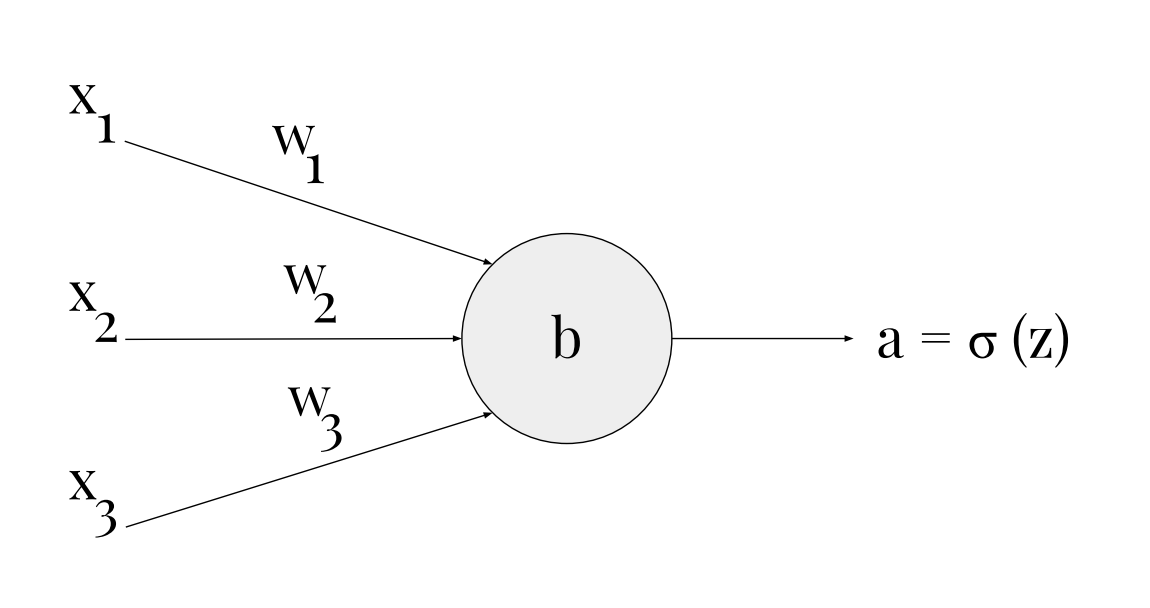
\includegraphics[width=8cm]{kapitel2/entropie.png}
    \caption[Darstellung der Kreuzentropie am beispiel eines Neurons]{Das Neuron wird mit 3 Eingabewerten $(x_1, x_2, x_3)$ den dazugehörigen Gewichten $(W_1, W_2, W_3)$ trainiert. Der Bias ist durch $b$ angegeben und die Ausgabe mit $a = \sigma(z)$ (in Anlehnung an \cite*{Nielsen2015})}
    \label{Kap2:Entropie}
\end{figure}

\section{Convolutional Neural Network}

ConvNets/CNNs oder \textit{Convolutional Neural Networks} dienen zur Verarbeitung von Daten in Form mehrerer Arrays, beispielsweise eines Farbbildes aus drei 2-dimensionalen Arrays mit Pixelintensitäten in den drei Farbkanälen. Viele Daten liegen in Form mehrerer Arrays vor: 1D für Signale und Sequenzen, einschließlich Sprache, 2D für Bilder oder Audio und 3D für Video. Hinter ConvNets stehen vier Schlüsselideen, die die Eigenschaften natürlicher Signale nutzen: lokale Verbindungen, gemeinsame Gewichte, Pooling und die Verwendung vieler Schichten \cite*{Lecun2015}. In den folgenden Abschnitten werden diese Konzepte näher erklärt.


CNNs arbeiten mit gitterstrukturierten Eingaben, die in lokalen Regionen des Netzes starke räumliche Abhängigkeiten aufweisen. Das offensichtlichste Beispiel für gitterstrukturierte Daten ist ein zweidimensionales Bild. Diese Art von Daten weisen räumliche Abhängigkeiten auf, da benachbarte räumliche Orte in einem Bild häufig ähnliche Farbwerte der einzelnen Pixel aufweisen. Eine zusätzliche Dimension erfasst die verschiedenen Farben, wodurch ein dreidimensionales Eingabevolumen entsteht. Andere Formen von sequentiellen Daten wie Text, Zeitreihen und Sequenzen können ebenfalls als Sonderfälle von Daten mit Gitterstruktur mit verschiedenen Arten von Beziehungen zwischen benachbarten Elementen betrachtet werden. Die überwiegende Mehrheit der Anwendungen von CNNs konzentriert sich auf Bilddaten, obwohl man diese Netze auch für alle Arten von zeitlichen und räumlichen Daten verwenden kann. Ein wichtiges definierendes Merkmal von CNNs ist eine Operation, die als Faltung (\enquote{convolution}) bezeichnet wird. \cite*[315-316]{Aggarwal2018}.




\subsection{Architektur}
In CNNs sind mehrere Schichten miteinander verbunden und jeder Schicht hat eine Gitterstruktur. Die Bezihungen zwischen den Schichten werden von einer Schicht zur nächsten vererbt, da jedes Merkmalswert aus einem kleinen lokalen Bereich aus der vorherigen Schicht basiert. Es ist wichtig, diese räumlichen Beziehungen zwischen den Gitterzellen aufrechtzuerhalten, da die Faltungsoperation und die Transformation zur nächsten Schicht von diesen Beziehungen abhängen. Jede Schicht im Faltungsnetzwerk ist eine dreidimensionale Gitterstruktur mit einer Höhe, Breite und Tiefe. Die Tiefe einer Schicht in einem Faltungsnetzwerk ist nicht die Tiefe des Netzwerks selbst. Das Wort \enquote{Tiefe} bezieht sich auf die Anzahl der Kanäle in jeder Ebene, z. B. die Anzahl der Primärfarbkanäle (z. B. Blau, Grün und Rot) im Eingabebild \cite*[318]{Aggarwal2018}.

Die Architektur eines typischen ConvNets ist in mehrere Phasen unterteilt. Die ersten Stufen bestehen aus zwei Arten von Schichten: Faltungsschichten und Poolschichten. Einheiten in einer Faltungsebene werden in sogenannten \enquote{Feature-Maps} organisiert, in denen jede Einheit über eine Reihe von Gewichten, die als \enquote{Filterbank} bezeichnet werden, mit lokalen Patches in den Feature-Maps der vorherigen Ebene verbunden ist. Das Ergebnis dieser lokal gewichteten Summe wird dann durch eine Nichtlinearität wie \zb eine ReLU geleitet. Alle Einheiten in einer Feature-Map verwenden dieselbe Filterbank\cite*{Lecun2015}.


\begin{figure}[H]
    \centering
    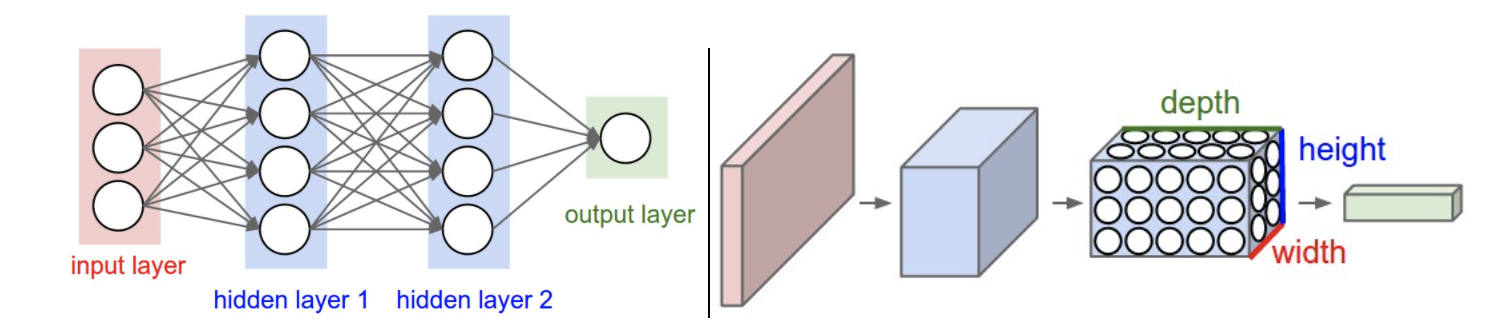
\includegraphics[width=13cm]{kapitel2/conv.png}
    \caption[Vergleich eines NN mit einem CNN]{Links: Ein reguläres 3-Schicht-Neuronales Netz. Rechts: Ein ConvNet. Es ordnet seine Neuronen in drei Dimensionen (Breite, Höhe, Tiefe) an, wie in einer der Ebenen dargestellt. Jede Schicht eines ConvNet wandelt das 3D-Eingangsvolumen in ein 3D-Ausgangsvolumen von Neuronenaktivierungen um. In diesem Beispiel enthält die rote Eingabeebene das Bild, sodass seine Breite und Höhe den Abmessungen des Bildes entsprechen. Die \enquote{Tiefe} sind die 3 Farbkanäle (rot, grün, blau) aus \cite*{StanfordUniversityCoursecs231n2018a}.}
    \label{Kap2:Conv}
\end{figure}


\subsection{Convolutional Layer}

Die Parameter der Convolutional Layer (Faltungsschicht) bestehen aus einer Reihe von \enquote{lernbaren} Filtern. Jedes dieser Filter ist räumlich klein (Breite und Höhe), erstreckt sich jedoch über die gesamte Tiefe des Eingangsvolumens. Beispielsweise könnte ein typischer Filter auf einer ersten Schicht eines ConvNet die Größe \textit{5 × 5 × 3} haben (d. H. 5 Pixel Breite und Höhe und 3 Tiefe, weil Bilder die Tiefe 3 haben, also die Farbkanäle). Während des Vorwärtsdurchlaufs wird jedes der Filter über die Breite und Höhe des Eingangsvolumens gefaltet und es werden die Punktprodukte zwischen den Einträgen des Filters und dem Eingang an einer beliebigen Position berechnet. Wenn der Filter über die Breite und Höhe des Eingangsvolumens gefaltet wird, wird eine zweidimensionale \enquote{Aktivierungskarte} (\enquote{feature map}) erstellt, die die Antworten dieses Filters an jeder räumlichen Position angeben. Intuitiv lernt die Filter, die aktiviert werden, wenn sie eine Art visuelles Merkmal sehen, z. B. eine Kante mit einer bestimmten Ausrichtung oder einen Farbfleck auf der ersten Ebene oder schließlich Muster auf höheren Ebenen des Netzwerks. Es entstehen somit ein ganzer Satz von Filtern in jeder Faltungsschicht (z. B. 12 Filter), und jeder von ihnen erzeugt eine separate zweidimensionale Aktivierungskarte. Diese Karten werden entlang der Tiefendimension gestapelt und das Ausgabevolumen erzeugt \cite*{StanfordUniversityCoursecs231n2018a}.

\begin{figure}[H]
    \centering
    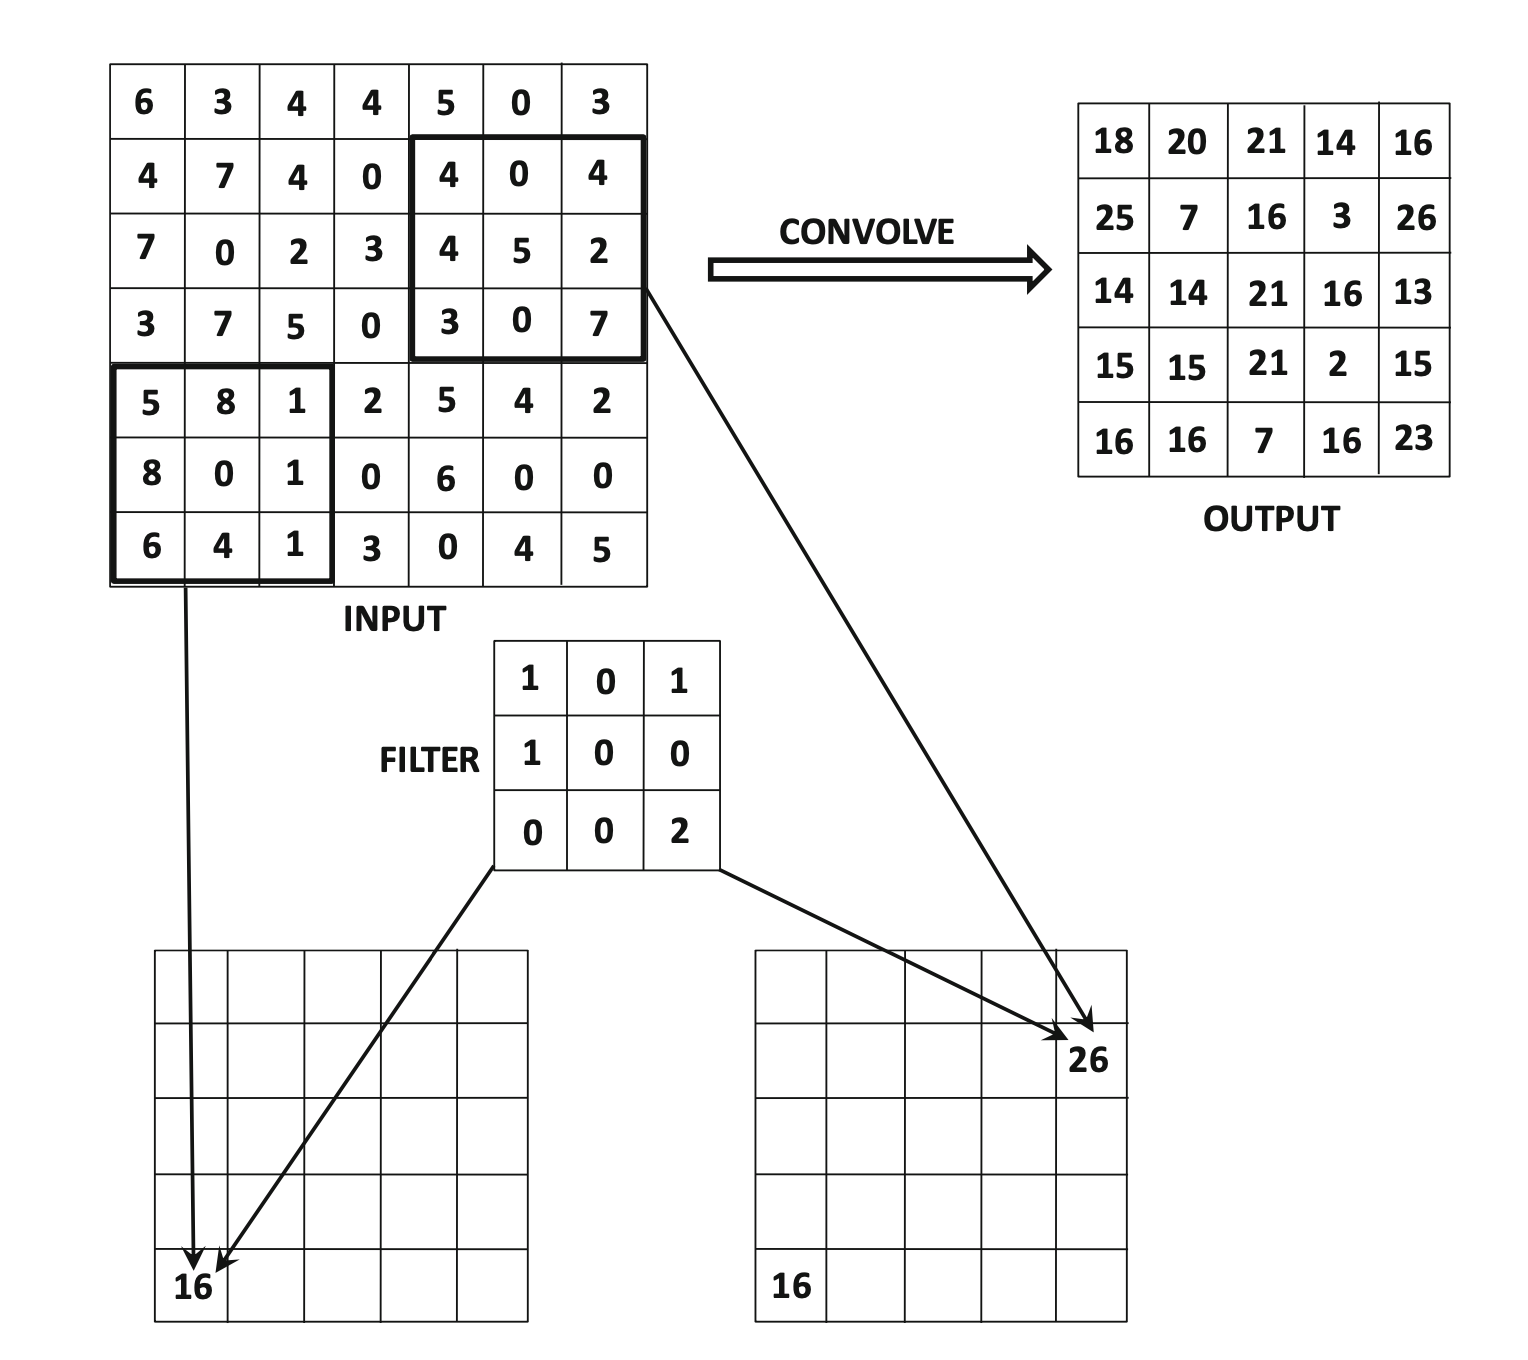
\includegraphics[width=10cm]{kapitel2/conv_layers.png}
    \caption[Die Faltung in einem CNN]{Die Faltungsoperation geschieht durch eine Punktprodukt Operation des Filters, was über alle räumlichen Positionen wiederholt wird aus \cite*[321]{Aggarwal2018}.}
    \label{Kap2:Conv}
\end{figure}

\subsection{Padding}
Die Faltungsoperation verringert die Größe der $(q + 1)$-ten Schicht im Vergleich zur Größe der $q$-ten Schicht. Diese Art der Größenreduzierung ist im Allgemeinen nicht wünschenswert, da sie dazu neigt, einige Informationen entlang der Ränder zu verlieren. Dieses Problem kann durch \textit{Padding} (\enquote{Auffüllen}) gelöst werden. Beim Padding werden neue Werte rund um die Ränder der Feature-Maps hinzugefügt. Der Wert jedes dieser aufgefüllten Feature-Werte wird auf 0 gesetzt. Diese Bereiche tragen nicht zum endgültigen Punktprodukt bei, da ihre Werte auf 0 gesetzt sind. Ein Teil des Filters aus den Rändern der Schicht wird \enquote{herausragt} und dann durch das Durchführen der Punktprodukt Operation, nur über den Teil der Ebene ersetzt, in dem Werte definiert sind \cite*[323]{Aggarwal2018}.


\subsection{Pooling}
Es ist üblich, regelmäßig eine \textit{Pooling Ebene} zwischen aufeinander folgenden Faltungsebenen einer ConvNet-Architektur einzufügen. Die Funktion dieser Ebenen besteht darin, die räumliche Größe der Darstellung schrittweise zu verringern, um die Anzahl der Parameter und die Berechnung im Netzwerk zu verringern und damit auch die Überanpassung zu steuern. Die Pooling-Ebene arbeitet unabhängig mit jedem Abschnitt der Eingabe und ändert die Größe räumlich. Die gebräuchlichste Form ist eine Pooling-Ebene mit Filtern der Größe \textit{2x2}, die mit einem  \enquote{Stride} von 2 Samples pro Scheibe in der Eingabe, um 2 entlang der Breite und Höhe angewendet werden, wobei 75\% der Aktivierungen verworfen werden \cite*{StanfordUniversityCoursecs231n2018a}.

\begin{figure}[H]
    \centering
    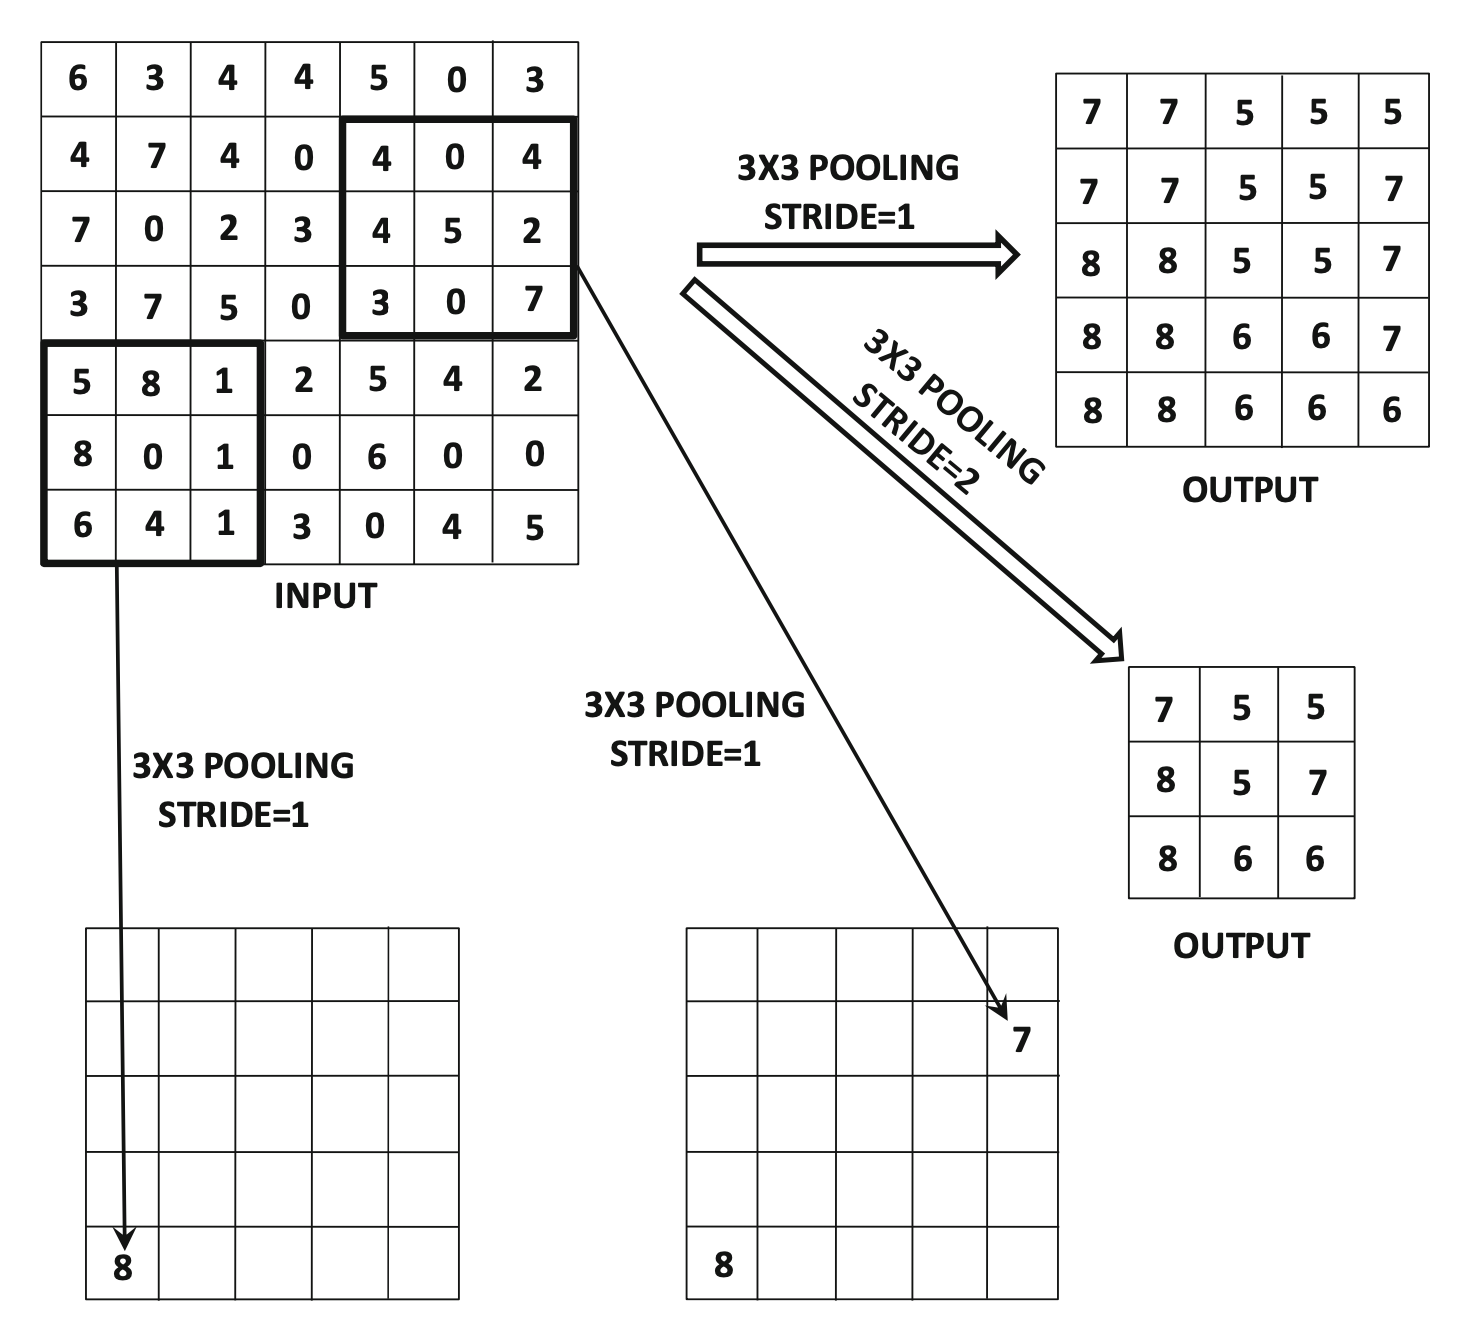
\includegraphics[width=9cm]{kapitel2/maxpooling.png}
    \caption[Max-Pooling]{Ein Beispiel für ein Max-Pooling einer Aktivierungskarte der Größe \textit{7 × 7} mit Stride von 1 und 2. Ein Stride von 1 erzeugt eine 5 × 5-Aktivierungskarte mit stark wiederholten Elementen aufgrund der Maximierung in überlappenden Regionen. Ein Stride von 2 erzeugt eine 3 × 3-Aktivierungskarte mit weniger Überlappung \cite*[326]{Aggarwal2018}.}
    \label{Kap2:Pooling}
\end{figure}


\subsection{Vollständig verbundene Ebenen}
Am Ende wird die sogenannte \textit{vollständig verbundene Ebenen} des Netzwerkes verwendet, um Klassenwerte zu berechnen, die als Ausgabe des Netzwerks dienen sollen. In einem traditionellen vorwärts gerichteten Neuronalen Netzwerk wird jedes Eingangsneuron mit jedem Ausgangsneuron in der nächsten Schicht verbunden. Dieses wird auch als vollständig verbundene Schicht bezeichnet. Der einzige Unterschied zwischen der vollständig verbundene Ebene und Faltungsschichten besteht darin, dass die Neuronen in der Faltungsschicht nur mit einer lokalen Region der Eingabe verbunden ist. Die Neuronen in beiden Schichten berechnen jedoch immer noch Punktprodukte, sodass ihre funktionale Form identisch ist. Zwischen beiden Schichten ist eine Konvertierung möglich \cite*{StanfordUniversityCoursecs231n2018a}.


